\documentclass[../Tesi.tex]{subfiles}


\begin{document}
\section{Descrizione dei package}
Di seguito vengono presentati i package che compongono l'applicazione. Le componenti riportate in colori differenti dal giallo sono evidenziate poiché appartenenti a librerie esterne.

	\subsection{Package model}
		\begin{figure}[H]
			\centering
			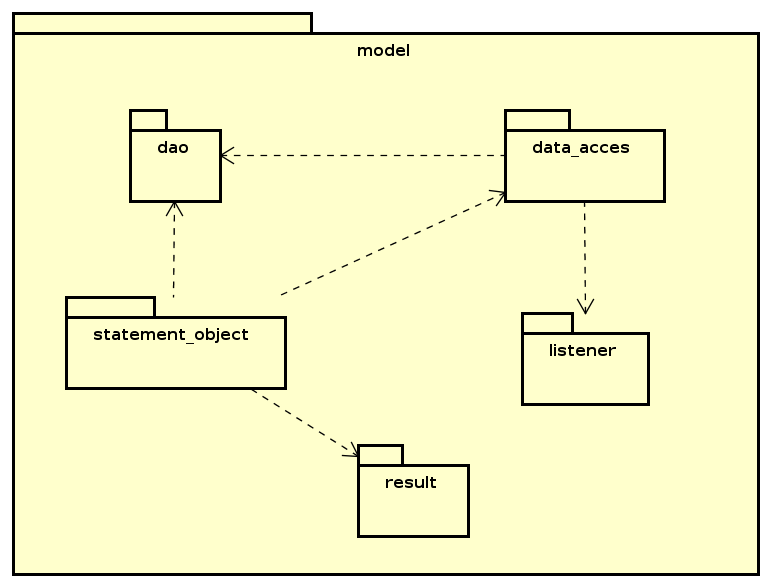
\includegraphics[scale=0.6]{images/package_diagrams/model}
				\caption{Package model}
		\end{figure}
		Il package \mpackage{model} racchiude tutte le componenti che si occupano della rappresentazione dei dati trattati dall'applicazione, della loro memorizzazione e recupero. \\
		I package contenuti al suo interno sono:
		\begin{itemize}
			\item \mpackage{dao};
			\item \mpackage{data\_access};
			\item \mpackage{statement\_object};
			\item \mpackage{listener};
			\item \mpackage{result}.
		\end{itemize}

	\subsection{Package model::dao}
		\begin{figure}[H]
			\centering
			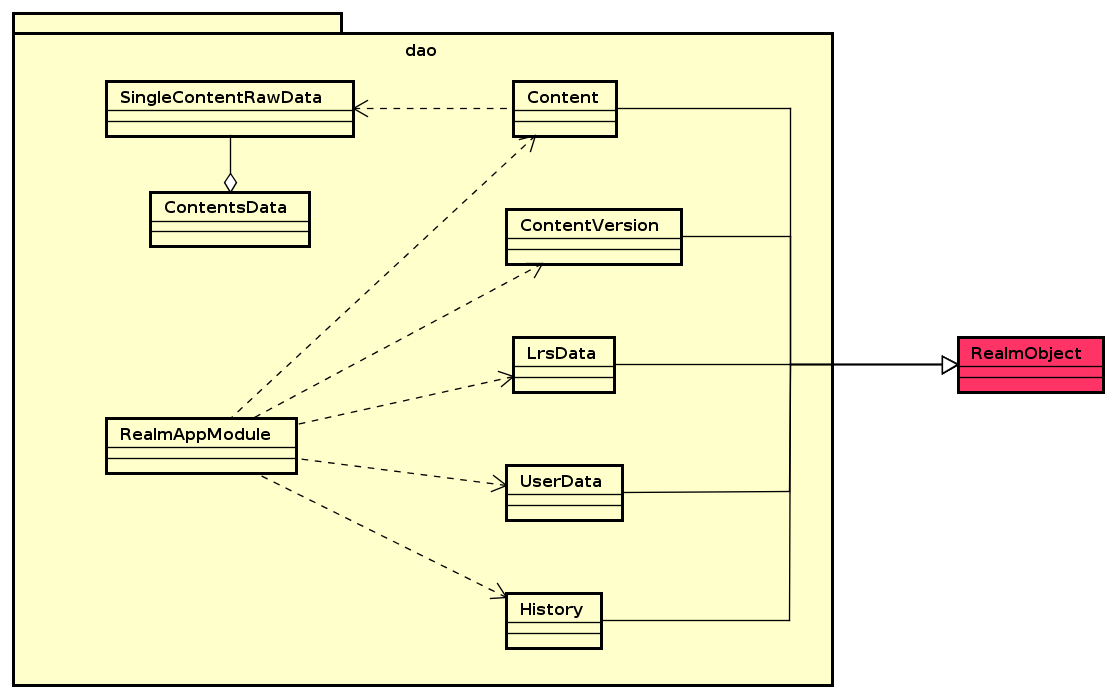
\includegraphics[scale=0.5]{images/package_diagrams/dao}
				\caption{Package dao}
		\end{figure}
		Il package \mpackage{dao} contiene tutte le componenti che si occupano della rappresentazione dei dati che vengono salvati nel database locale al dispositivo. Tutte le classi al suo interno corrispondono alle tabelle del database, ad eccezione delle classi \mclass{SingleContentRawData} e \mclass{ContentsData}, che sono utili al recupero delle informazioni necessarie per la creazione di oggetti di tipo \mclass{Content}, e della classe \mclass{RealmAppModule}. Tali classi estendono tutte \mclass{RealmObject} poiché, in questo modo, possono essere salvate direttamente all'interno del database locale utilizzando la libreria Realm. \\
		Le classi che appartengono a tale package sono:
		\begin{itemize}
			\item \mclass{Content};
			\item \mclass{ContentVersion};
			\item \mclass{History};
			\item \mclass{UserData};
			\item \mclass{LrsAccessData};
			\item \mclass{SingleContentRawData};
			\item \mclass{ContentsData};
			\item \mclass{RealmAppModule}.
		\end{itemize}

	\subsection{Package model::data\_access}
		\begin{figure}[H]
			\centering
			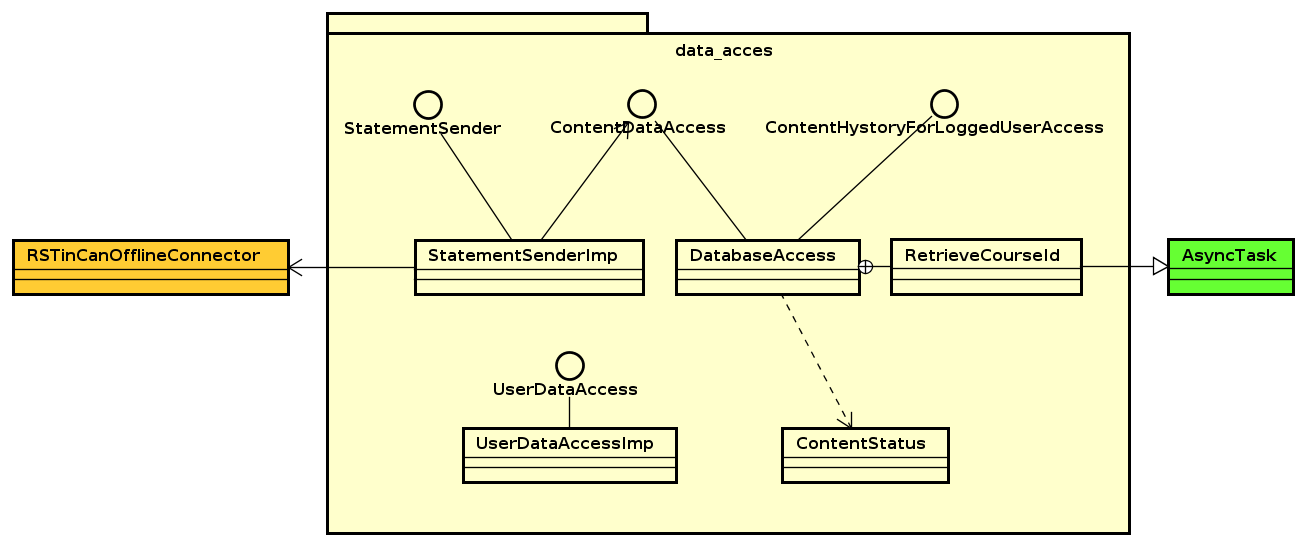
\includegraphics[scale=0.4]{images/package_diagrams/data_access}
				\caption{Package data\_access}
		\end{figure}
		Il package \mpackage{data\_access} contiene tutte le componenti che si occupano dell'accesso e della modifica dei dati salvati nel database interno al dispositivo. \\
		Le interfacce che appartengono a tale package sono:
		\begin{itemize}
			\item \mclass{StatementSender};
			\item \mclass{ContentDataAccess};
			\item \mclass{ContentHystoryForLoggedUserAccess};
			\item \mclass{UserDataAccess}.
		\end{itemize}
		Le classi che appartengono a tale package sono:
		\begin{itemize}
			\item \mclass{ContentStatus};
			\item \mclass{DatabaseAccess};
			\item \mclass{DatabaseAccess.RetrieveCourseId};
			\item \mclass{StatementSenderImp};
			\item \mclass{UserDataAccessImp}.
		\end{itemize}

	\subsection{Package model::listener}
		\begin{figure}[H]
			\centering
			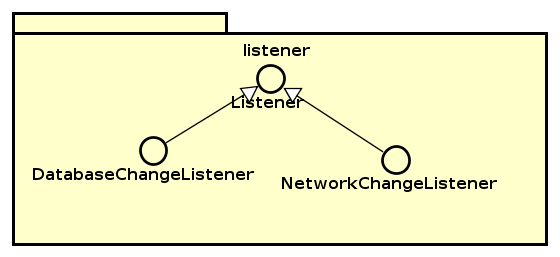
\includegraphics[scale=0.6]{images/package_diagrams/listener}
				\caption{Package listener}
		\end{figure}
		Il package \mpackage{listener} contiene tutte le interfacce che devono essere implementate dalle classi che vogliono essere registrate come listener. \\
		Le interfacce che appartengono a tale package sono:
		\begin{itemize}
			\item \mclass{Listener};
			\item \mclass{DatabaseChangeListener};
			\item \mclass{NetworkChangeListener}.
		\end{itemize}

	\subsection{Package model::result}
		\begin{figure}[H]
			\centering
			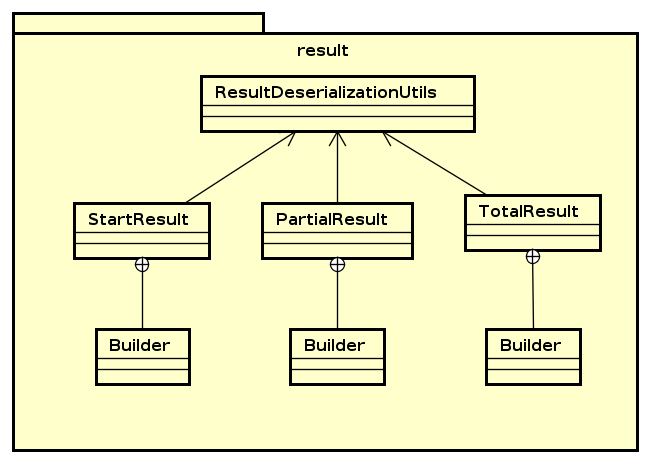
\includegraphics[scale=0.6]{images/package_diagrams/result}
				\caption{Package result}
		\end{figure}
		Il package \mpackage{result} contiene tutte le classi che si occupano della trasformazione di oggetti in formato JSON, i quali rappresentano i dati delle interazioni di un utente con un certo contenuto xAPI che devono essere registrati, in oggetti Java. \\
		Le classi che appartengono a tale package sono:
		\begin{itemize}
			\item \mclass{PartialResult};
			\item \mclass{PartialResult.Builder};
			\item \mclass{StartResult};
			\item \mclass{StartResult.Builder};
			\item \mclass{TotalResult};
			\item \mclass{TotalResult.Builder};
			\item \mclass{ResultDeserializationUtilities}.
		\end{itemize}

	\subsection{Package model::lrs\_access}
		\begin{figure}[H]
			\centering
			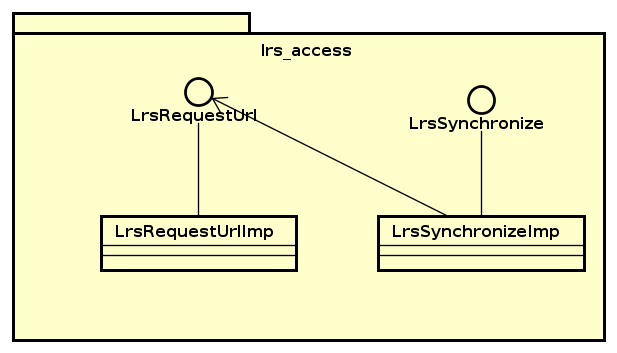
\includegraphics[scale=0.6]{images/package_diagrams/lrs_access}
				\caption{Package lrs\_access}
		\end{figure}
		Il package \mpackage{lrs\_access} contiene tutte le componenti che si occupano di effettuare delle richieste ad un LRS al fine di recuperare informazioni riguardanti un determinato utente. \\
		Le interfacce che appartengono a tale package sono:
		\begin{itemize}
			\item \minterface{LrsRequestUrl};
			\item \minterface{LrsSynchronize}.
		\end{itemize}
		Le classi che appartengono a tale package sono:
		\begin{itemize}
			\item \mclass{LrsRequestUrlImp};
			\item \mclass{LrsSynchronizeImp}.
		\end{itemize}

	\subsection{Package model::statement\_object}
		\begin{figure}[H]
			\centering
			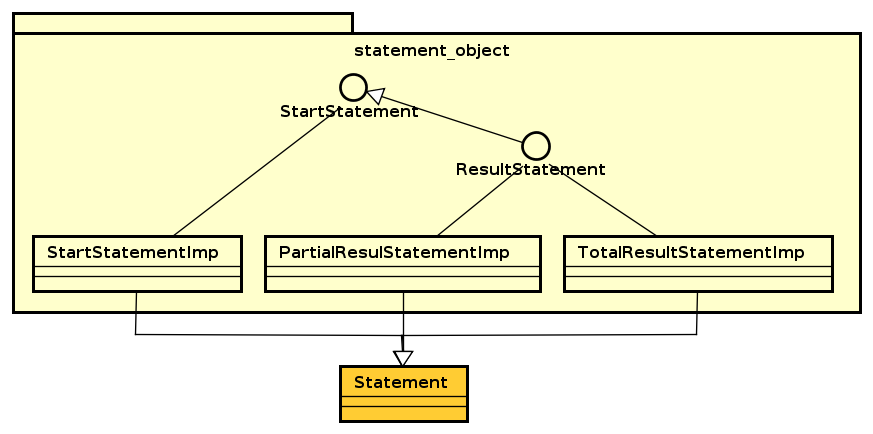
\includegraphics[scale=0.6]{images/package_diagrams/statement_object}
				\caption{Package statement\_object}
		\end{figure}
		Il package \mpackage{statement\_object} contiene tutte le componenti che servono per la rappresentazione di statement xAPI che devono essere inviati ad un LRS.\\
		Le interfacce che appartengono a tale package sono:
		\begin{itemize}
			\item \minterface{StartStatement};
			\item \minterface{ResultStatement}.
		\end{itemize}
		Le classi che appartengono a tale package sono:
		\begin{itemize}
			\item \mclass{StartStatementImp};
			\item \mclass{PartialResultStatement};
			\item \mclass{TotalResultStatement}.
		\end{itemize}

	\subsection{Package presenter}
		\begin{figure}[H]
			\centering
			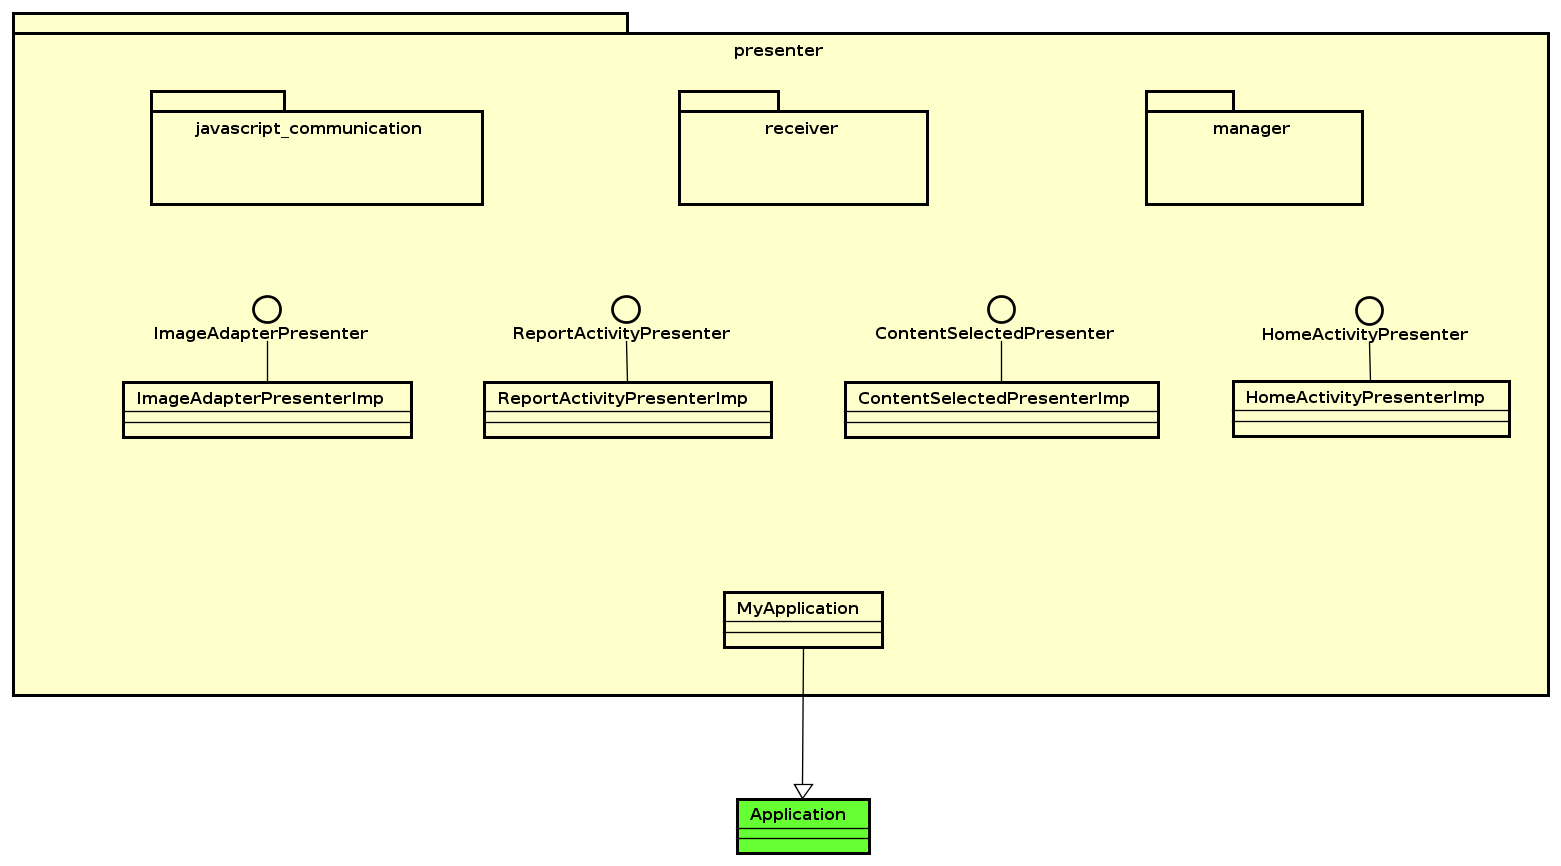
\includegraphics[scale=0.4]{images/package_diagrams/presenter}
				\caption{Package presenter}
		\end{figure}
		Il package \mpackage{presenter} contiene tutte le componenti che si occupano della comunicazione tra i package \mpackage{model} e \mpackage{view}. \\
		I package contenuti al suo interno sono:
		\begin{itemize}
			\item \mpackage{javascript\_communication};
			\item \mpackage{manager};
			\item \mpackage{receiver}.
		\end{itemize}
		Le interfacce che appartengono a tale package sono:
		\begin{itemize}
			\item \minterface{ContentSelectedPresenter};
			\item \minterface{HomeActivityPresenter};
			\item \minterface{ImageAdapterPresenter};
			\item \minterface{ReportActivityPresenter}.
		\end{itemize}
		Le classi che appartengono a tale package sono:
		\begin{itemize}
			\item \mclass{ContentSelectedPresenterImp};
			\item \mclass{HomeActivityPresenterImp};
			\item \mclass{ImageAdapterPresenterImp};
			\item \mclass{MyApplication};
			\item \mclass{ReportActivityPresenterImp}.
		\end{itemize}

	\subsection{Package presenter::javascript\_communication}
		\begin{figure}[H]
			\centering
			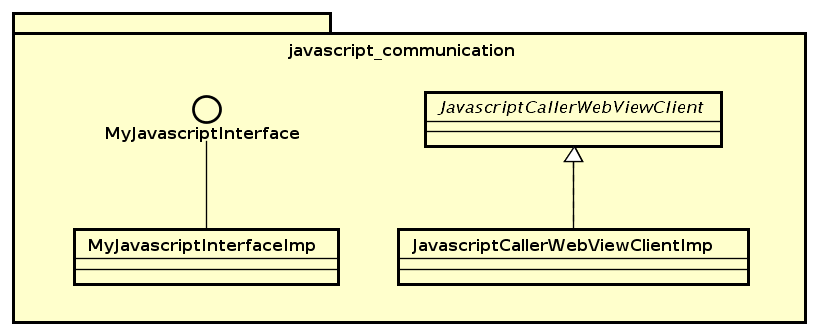
\includegraphics[scale=0.5]{images/package_diagrams/javascript_communication}
				\caption{Package javascript\_communication}
		\end{figure}
		Il package \mpackage{javascript\_communication} ha il compito di dialogare con gli script JavaScript che si occupano della gestione dei contenuti xAPI. \\
		Le interfacce che appartengono a tale package sono:
		\begin{itemize}
			\item \minterface{MyJavascriptInterface}.
		\end{itemize}
		Le classi che appartengono a tale package sono:
		\begin{itemize}
			\item \mclass{JavascriptCallerWebViewClient};
			\item \mclass{JavascriptCallerWebViewClientImp};
			\item \mclass{MyJavascriptInterface}.
		\end{itemize}

	\subsection{Package presenter::manager}
		\begin{figure}[H]
			\centering
			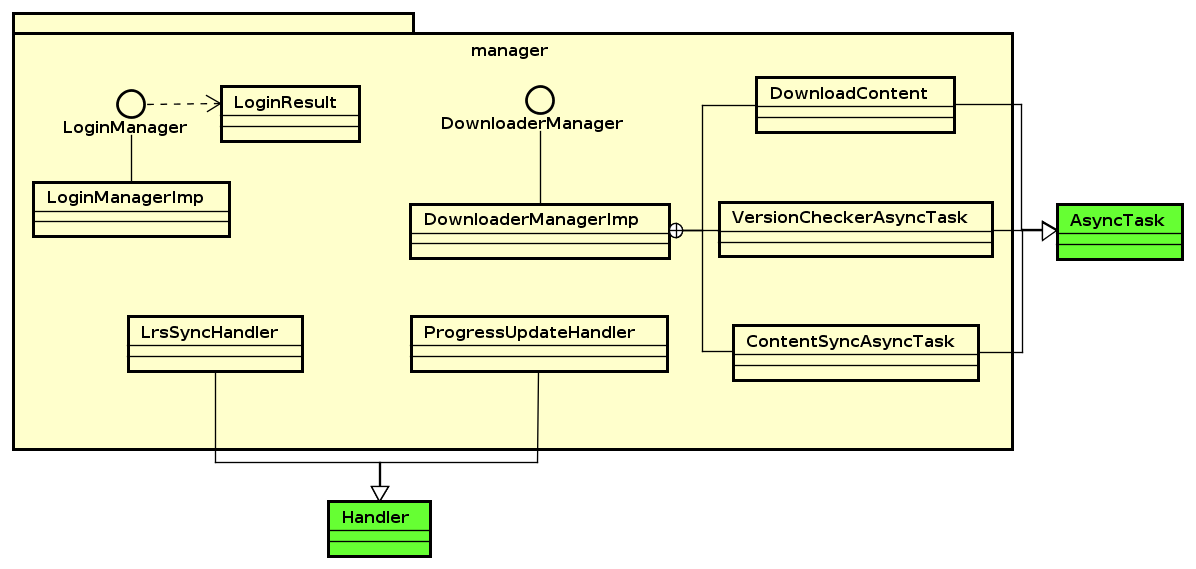
\includegraphics[scale=0.4]{images/package_diagrams/manager}
				\caption{Package manager}
		\end{figure}
		Il package \mpackage{manager} si occupa di effettuare delle connessioni a server in background per permettere il download dei contenuti oppure l'autenticazione e la registrazione di un utente. Al termine di una connessione ha il compito di aggiornare view e model. \\
		Le interfacce che appartengono a tale package sono:
		\begin{itemize}
			\item \minterface{DownloaderManager};
			\item \minterface{LoginManager}.
		\end{itemize}
		Le classi che appartengono a tale package sono:
		\begin{itemize}
			\item \mclass{DownloaderManagerImp};
			\item \mclass{DownloaderManagerImp.ContentSyncAsyncTask};
			\item \mclass{DownloaderManagerImp.DownloadContent};
			\item \mclass{DownloaderManagerImp.VersionCheckerAsyncTask};
			\item \mclass{LoginManagerImp};
			\item \mclass{LoginResult};
			\item \mclass{LrsSyncHandler};
			\item \mclass{ProgressUpdateHandler}.
		\end{itemize}

	\subsection{Package presenter::receiver}
		\begin{figure}[H]
			\centering
			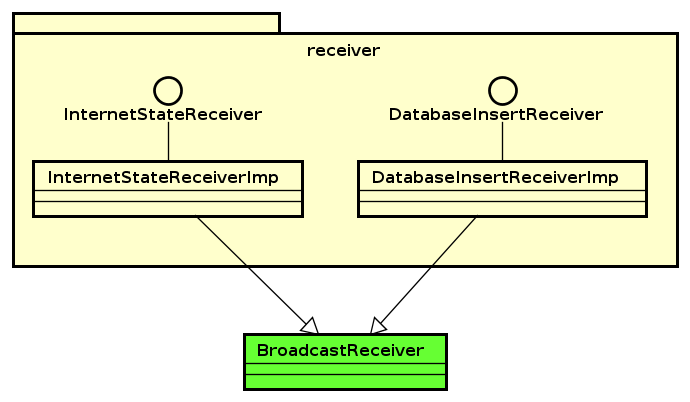
\includegraphics[scale=0.6]{images/package_diagrams/receiver}
				\caption{Package receiver}
		\end{figure}
		Il package \mpackage{receiver} si occupa di monitorare lo stato del database offerto dalla libreria TinCanAndroid-Offline e lo stato della connessione internet del dispositivo. \\
		Le interfacce che appartengono a tale package sono:
		\begin{itemize}
			\item \minterface{InternetStateReceiver};
			\item \minterface{DatabaseInsertReceiver}.
		\end{itemize}
		Le classi che appartengono a tale package sono:
		\begin{itemize}
			\item \mclass{InternetStateReceiverImp};
			\item \mclass{DatabaseInsertReceiverImp}.
		\end{itemize}

	\subsection{Package view}
		\begin{figure}[H]
			\centering
			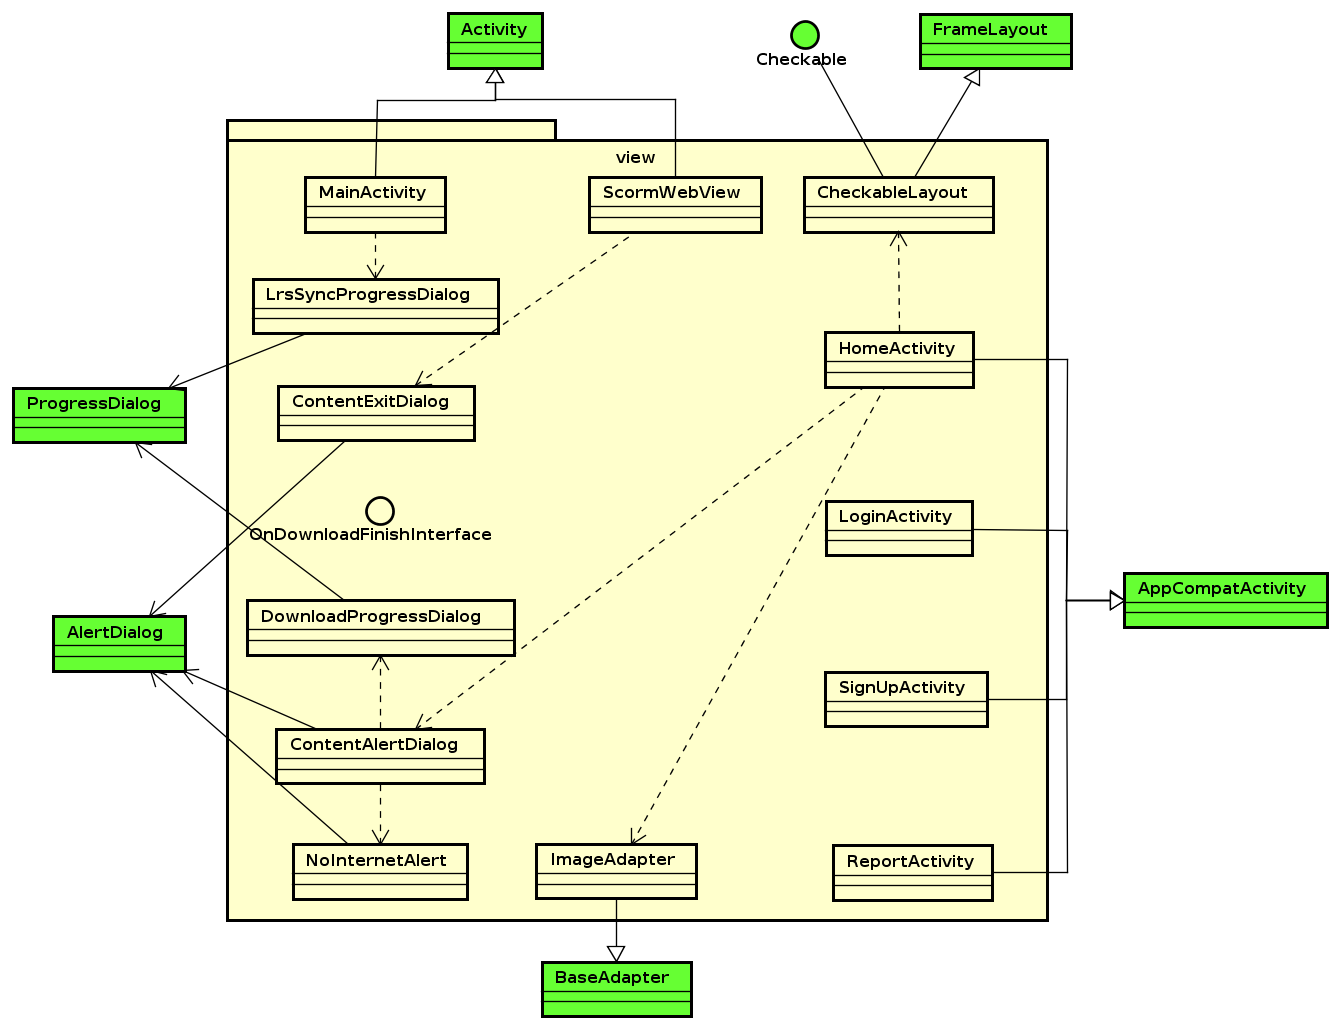
\includegraphics[scale=0.4]{images/package_diagrams/view}
				\caption{Package view}
		\end{figure}
		Il package \mpackage{view} si occupa dell'interfaccia grafica dell'applicazione. \\
		Le classi che appartengono a tale package sono:
		\begin{itemize}
			\item \mclass{CheckableLayout};
			\item \mclass{ContentAlertDialog};
			\item \mclass{ContentExitDialog};
			\item \mclass{DownloadProgressDialog};
			\item \mclass{HomeActivity};
			\item \mclass{ImageAdapter};
			\item \mclass{LoginActivity};
			\item \mclass{LrsSyncProgressDialog};
			\item \mclass{MainActivity};
			\item \mclass{NoInternetAlert};
			\item \mclass{ReportActivity};
			\item \mclass{ScormWebView};
			\item \mclass{SignUpActivity};
		\end{itemize}

	\subsection{Package dependency\_injection}
		\begin{figure}[H]
			\centering
			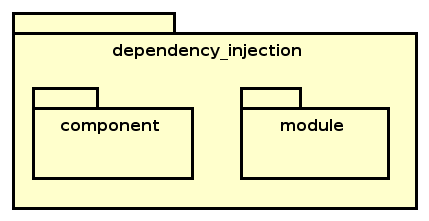
\includegraphics[scale=0.6]{images/package_diagrams/dependency_injection}
				\caption{Package dependency\_injection}
		\end{figure}
		Il package \mpackage{dependency\_injection} è il package nel quale vengono dichiarate quali classi necessitano dell'``iniezione'' di qualche campo e il modo di risolvere tali dipendenze. \\
		I package contenuti al suo interno sono:
		\begin{itemize}
			\item \mpackage{component};
			\item \mpackage{module}.
		\end{itemize}

	\subsection{Package dependency\_injection::component}
		\begin{figure}[H]
			\centering
			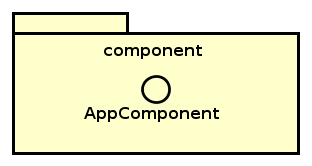
\includegraphics[scale=0.6]{images/package_diagrams/component}
				\caption{Package component}
		\end{figure}
		Il package \mpackage{component} è il package nel quale vengono dichiarate quali classi necessitano dell'``iniezione'' di qualche campo. \\
		Le interfacce che appartengono a tale package sono:
		\begin{itemize}
			\item \minterface{AppComponent}.
		\end{itemize}	

	\subsection{Package dependency\_injection::module}
		\begin{figure}[H]
			\centering
			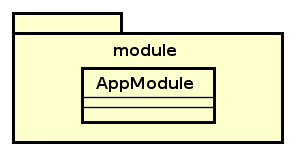
\includegraphics[scale=0.6]{images/package_diagrams/module}
				\caption{Package module}
		\end{figure}
		Il package \mpackage{module} è il package nel quale viene dichiarato come risolvere le dipendenze delle classi dichiarate nel package \mpackage{component}. \\
		Le classi che appartengono a tale package sono:
		\begin{itemize}
			\item \mclass{AppModule}.
		\end{itemize}

\end{document}